\documentclass[11pt]{article}

\usepackage[margin=1in]{geometry}
\usepackage{amsmath,amssymb,booktabs,graphicx,float,array}
\usepackage[dvipsnames]{xcolor}
\usepackage{hyperref}
\usepackage{setspace}
\usepackage{caption}

\hypersetup{
    colorlinks=true,
    linkcolor=MidnightBlue,
    urlcolor=MidnightBlue,
    citecolor=MidnightBlue
}

\setstretch{1.08}

\title{\textbf{RFF Complexity, Rolling Grassmann Diagnostics, and the Instability of Standard IPCA}}
\author{}
\date{}

\begin{document}

\maketitle

\section{Purpose of this note}

This note turns the uploaded RFF--IPCA output into a readable research-style summary with figures and interpretation.
The central question is not only whether complexity improves \emph{portfolio performance}, but also whether it improves the
\emph{geometric stability} of the induced factor subspaces. That distinction matters because the virtue-of-complexity literature
and the Grassmann-geometry framing are answering slightly different questions:

\begin{itemize}
    \item the \textbf{virtue-of-complexity} argument asks whether richer nonlinear models improve out-of-sample performance,
    \item the \textbf{geometry} argument asks whether the added flexibility expands the economically relevant return span in a stable way.
\end{itemize}

The uploaded results suggest a nuanced answer: \textbf{Sharpe ratio improves with RFF complexity, but the geometric diagnostics do not improve monotonically.}
That is precisely the regime in which a parameter-space IPCA estimator is a poor object to trust.

\section{Model idea}

We can view the lifted IPCA specification as
\begin{equation}
r_t \approx \Phi(Z_t)\Gamma^\top f_t + \varepsilon_t,
\end{equation}
where $Z_t$ are characteristics, $\Phi(Z_t)$ is a Random Fourier Feature (RFF) lift, $\Gamma$ maps lifted features into factor loadings,
and $f_t$ are latent factor returns.

The key geometric object is not the raw parameter matrix $\Gamma$, but the induced return subspace
\begin{equation}
V_t = \mathrm{span}\!\left(\Phi(Z_t)\Gamma^\top\right).
\end{equation}
Two different parameter matrices can generate nearly the same fitted return span. Once the lifted representation becomes rich,
the estimation problem is better understood as a \emph{subspace estimation problem} than a raw coefficient estimation problem.

\section{Headline empirical findings}

From the uploaded summary pages, the main results are:

\begin{table}[H]
\centering
\begin{tabular}{>{\raggedright\arraybackslash}p{2.1in}ccc}
\toprule
Model & Sharpe & Effective Rank & Grassmann Distance \\
\midrule
No RFF & 0.73 & 1.421 & 0.885 \\
RFF = 100 & 0.75 & 4.035 & 1.300 \\
RFF = 1000 & 0.82 & 1.706 & 2.047 \\
RFF = 2000 & 1.09 & -- & -- \\
\bottomrule
\end{tabular}
\caption{Summary metrics extracted from the uploaded result PDF.}
\end{table}

These numbers already tell the main story.

\subsection*{Performance story}
Sharpe rises from roughly $0.73$ without RFF to roughly $1.09$ at RFF = 2000. So at the level of portfolio performance,
the uploaded experiment is consistent with the virtue of complexity.

\subsection*{Geometry story}
The geometric quantities do \emph{not} move monotonically in the same direction. Effective rank is actually highest at RFF = 100,
while Grassmann distance is substantially larger for RFF = 1000 than for the no-RFF baseline. This means that added nonlinear flexibility
does not automatically translate into a cleaner or more persistent return-span expansion.

\section{Why this matters}

If one looked only at Sharpe ratio, the obvious conclusion would be that more nonlinear lifting is simply better.
But the rolling subspace plots show that some of this added flexibility may be entering through weakly identified directions that rotate over time.
That is the central distinction between

\begin{itemize}
    \item \textbf{economic virtue} of complexity: better out-of-sample performance,
    \item \textbf{geometric virtue} of complexity: stable expansion of intrinsic return dimension.
\end{itemize}

The uploaded evidence supports the first claim strongly, but supports the second only partially.

\section{Figures: cleaned summaries and extracted result panels}

Figure~\ref{fig:sharpe} and Figure~\ref{fig:geomsummary} summarize the main quantitative pattern in a cleaner way.
The following extracted result panels preserve the original output exactly as it appeared in the uploaded file.

\begin{figure}[H]
\centering
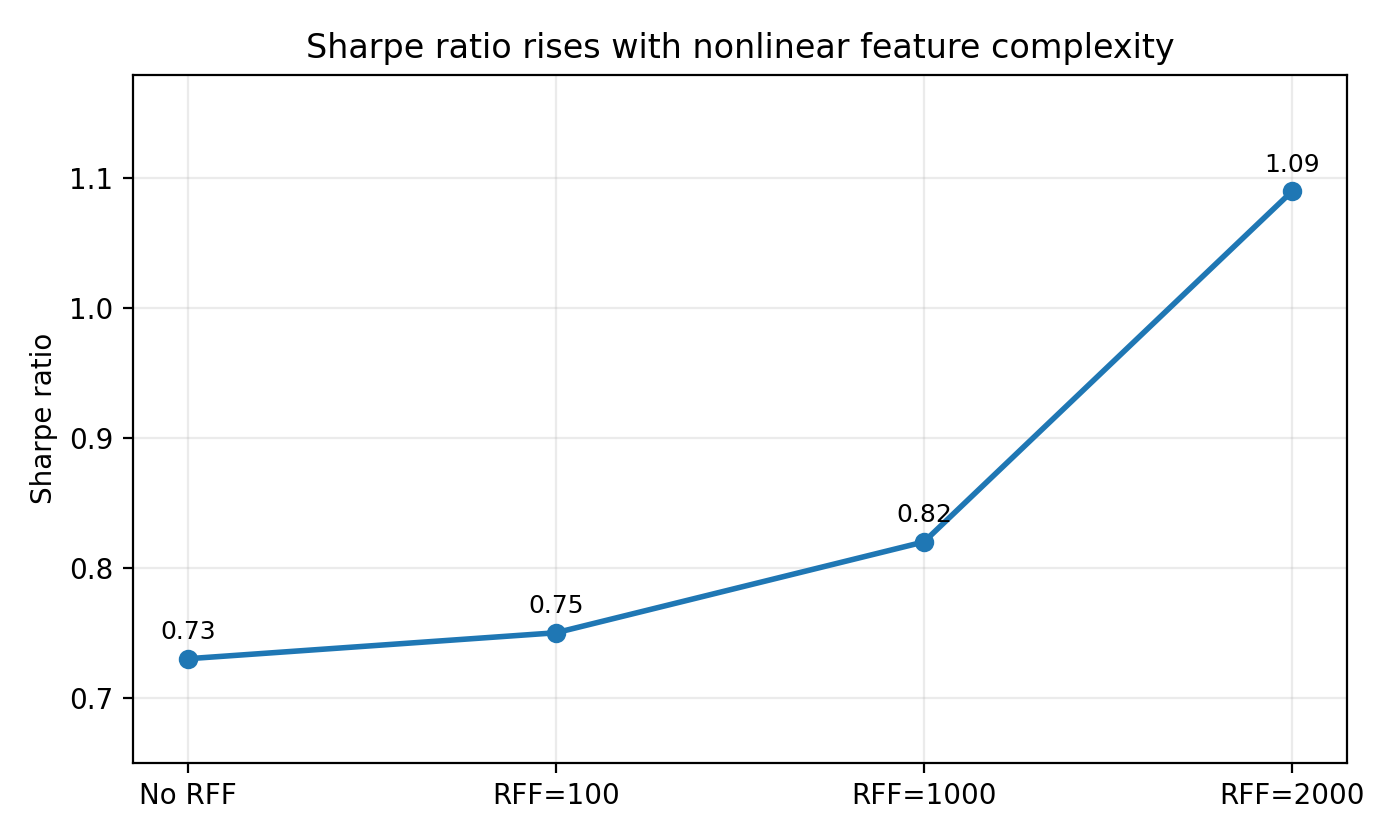
\includegraphics[width=0.78\textwidth]{figures/sharpe_trend.png}
\caption{Sharpe ratio versus model complexity. The upward trend supports the virtue of complexity in portfolio performance.}
\label{fig:sharpe}
\end{figure}

\begin{figure}[H]
\centering
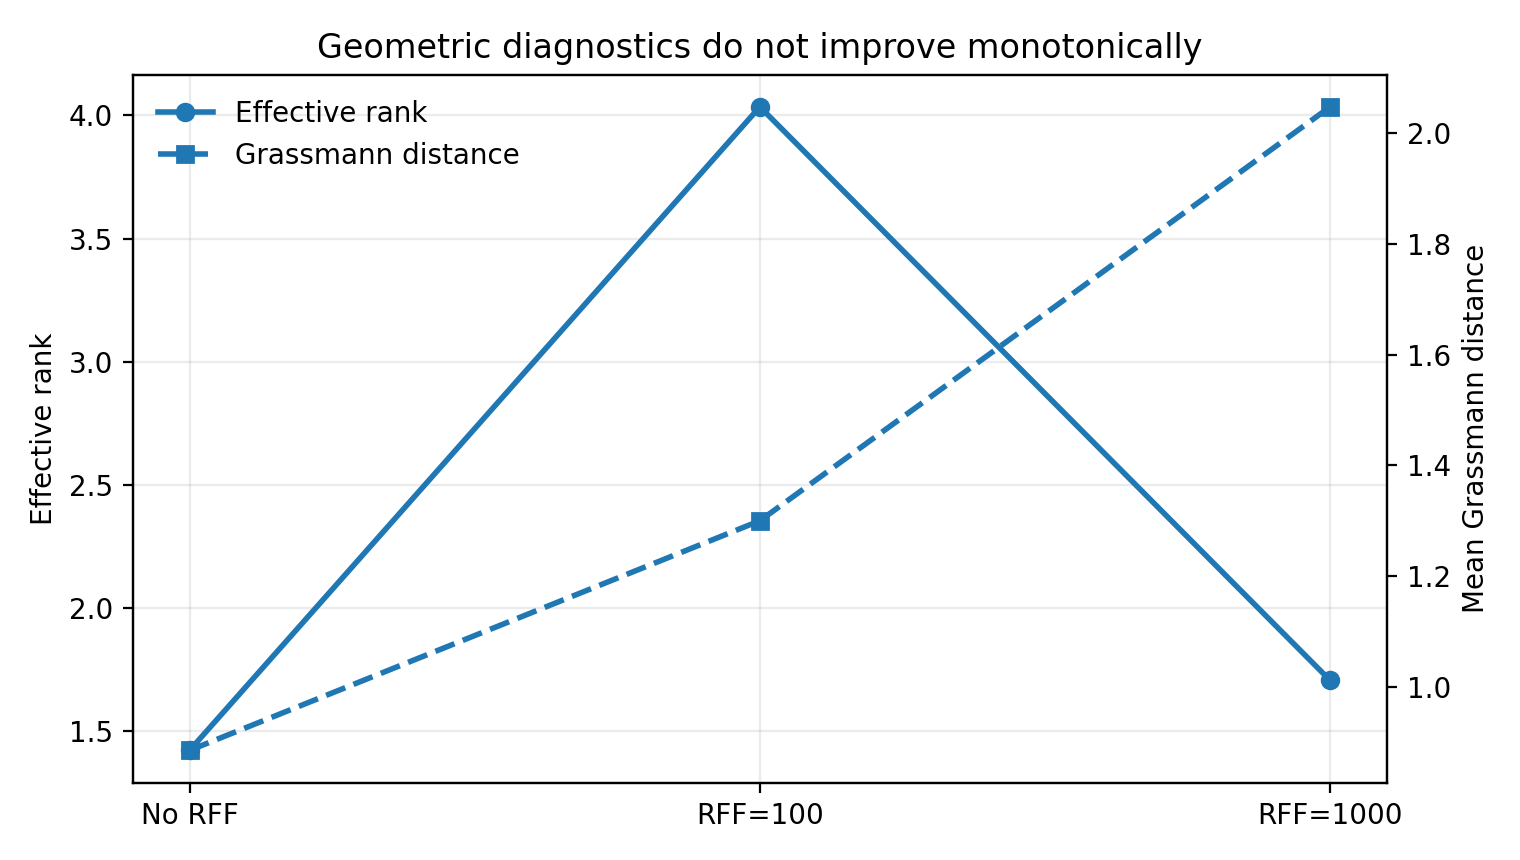
\includegraphics[width=0.82\textwidth]{figures/geometry_summary.png}
\caption{Summary geometric diagnostics. Effective rank and Grassmann distance do not improve monotonically as complexity rises.}
\label{fig:geomsummary}
\end{figure}

\begin{figure}[H]
\centering
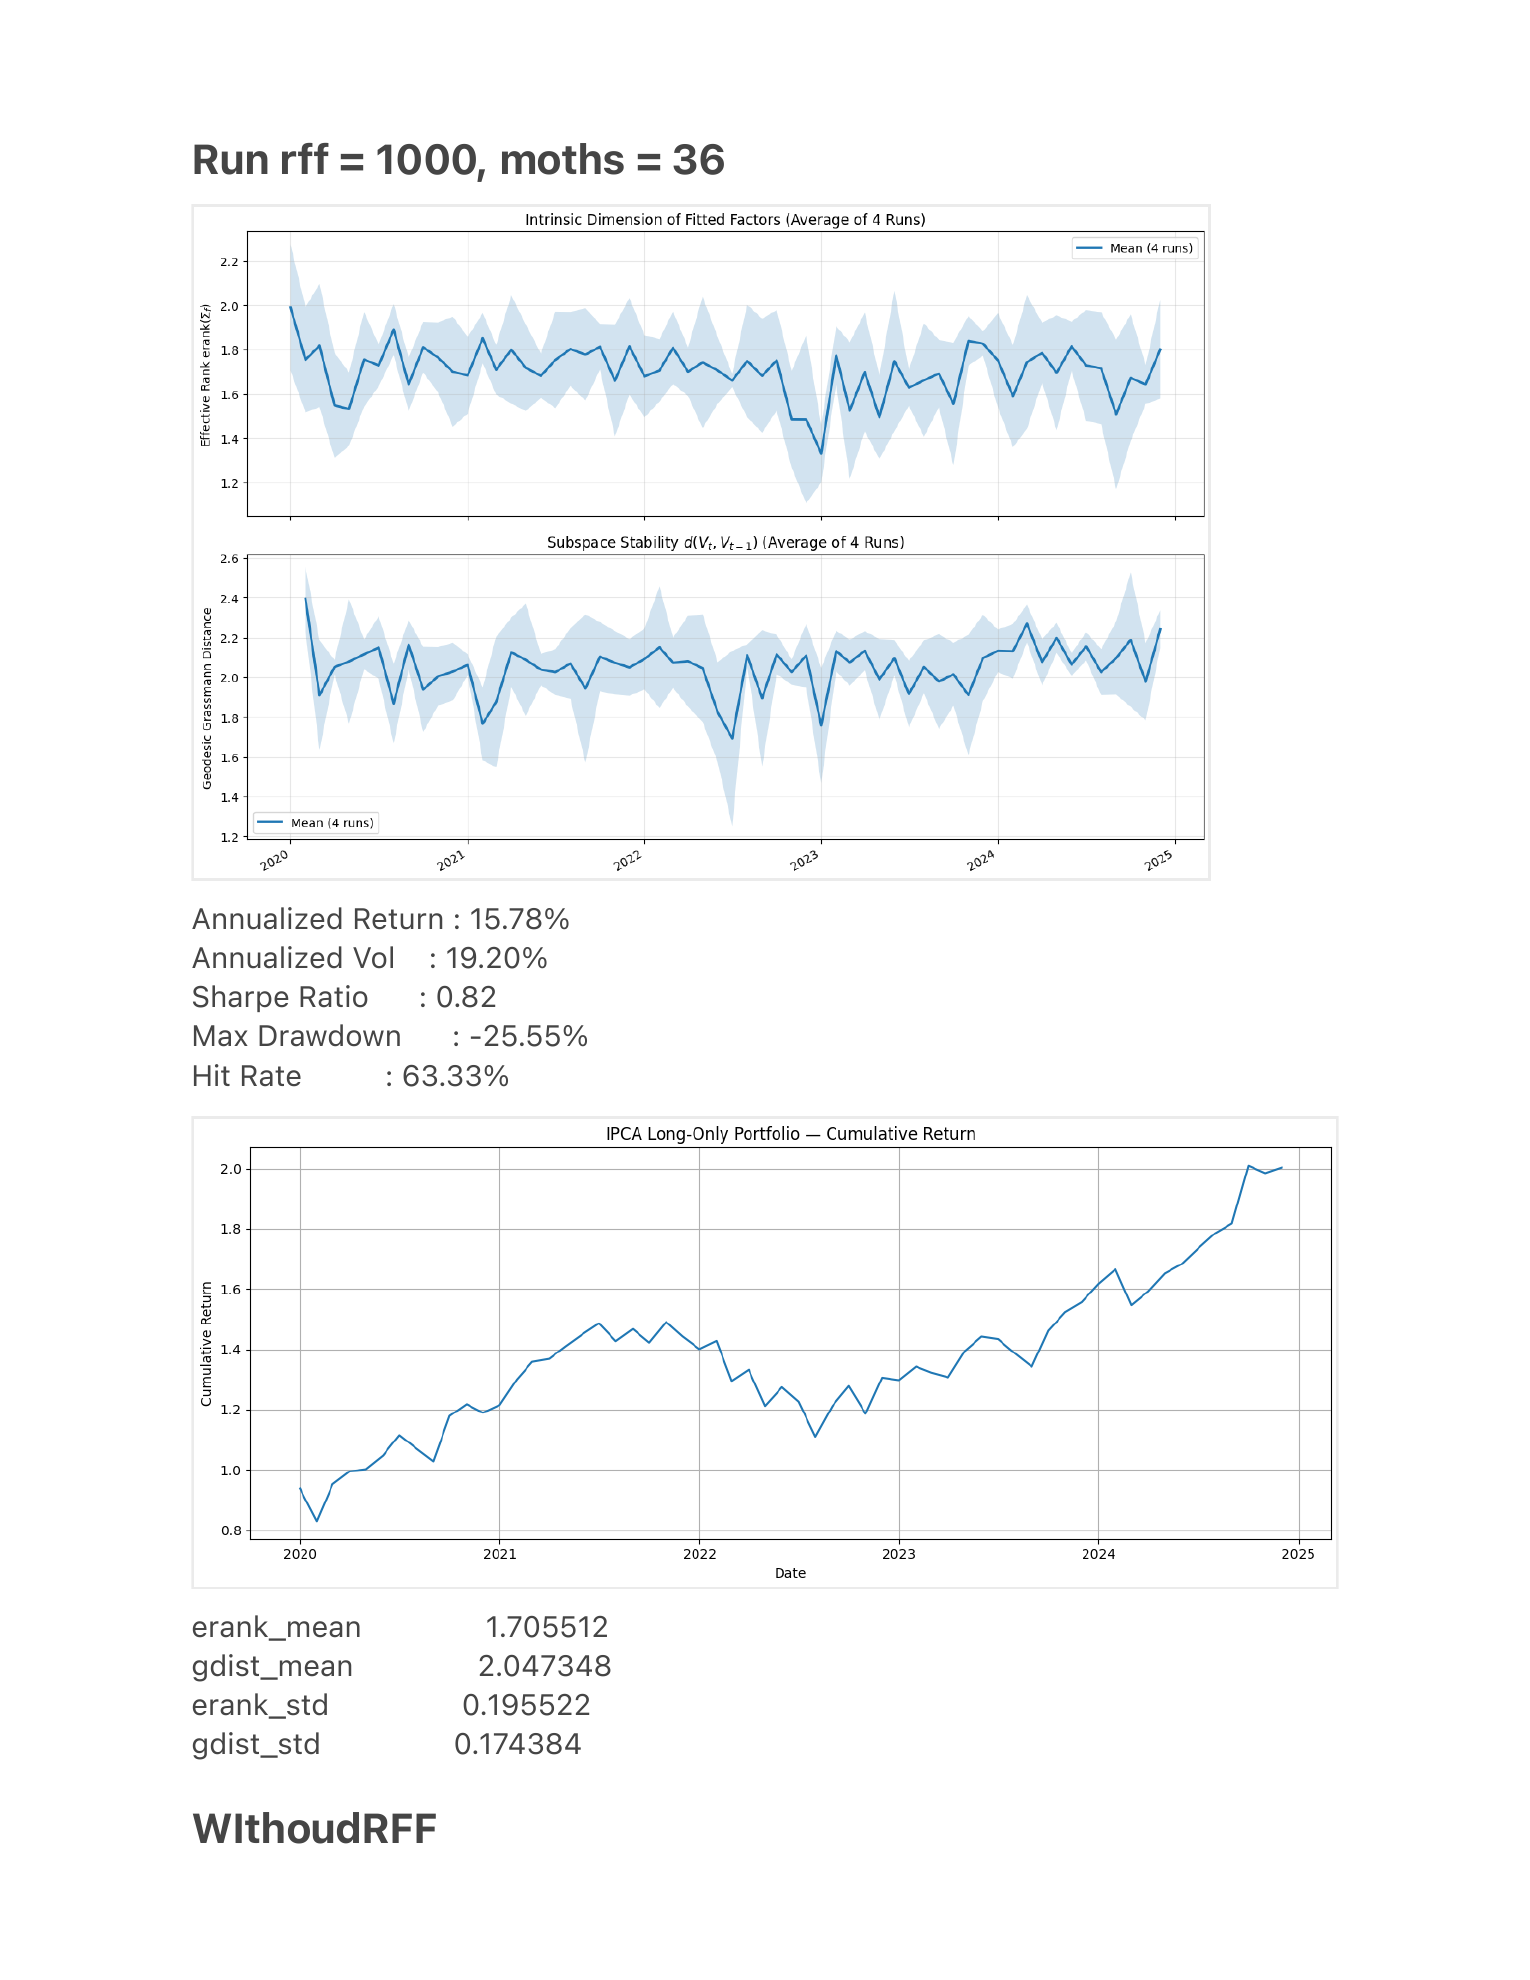
\includegraphics[width=0.88\textwidth]{figures/results_page1.png}
\caption{Extracted panel from the uploaded PDF: RFF = 1000 summary and comparison to the baseline.}
\end{figure}

\begin{figure}[H]
\centering
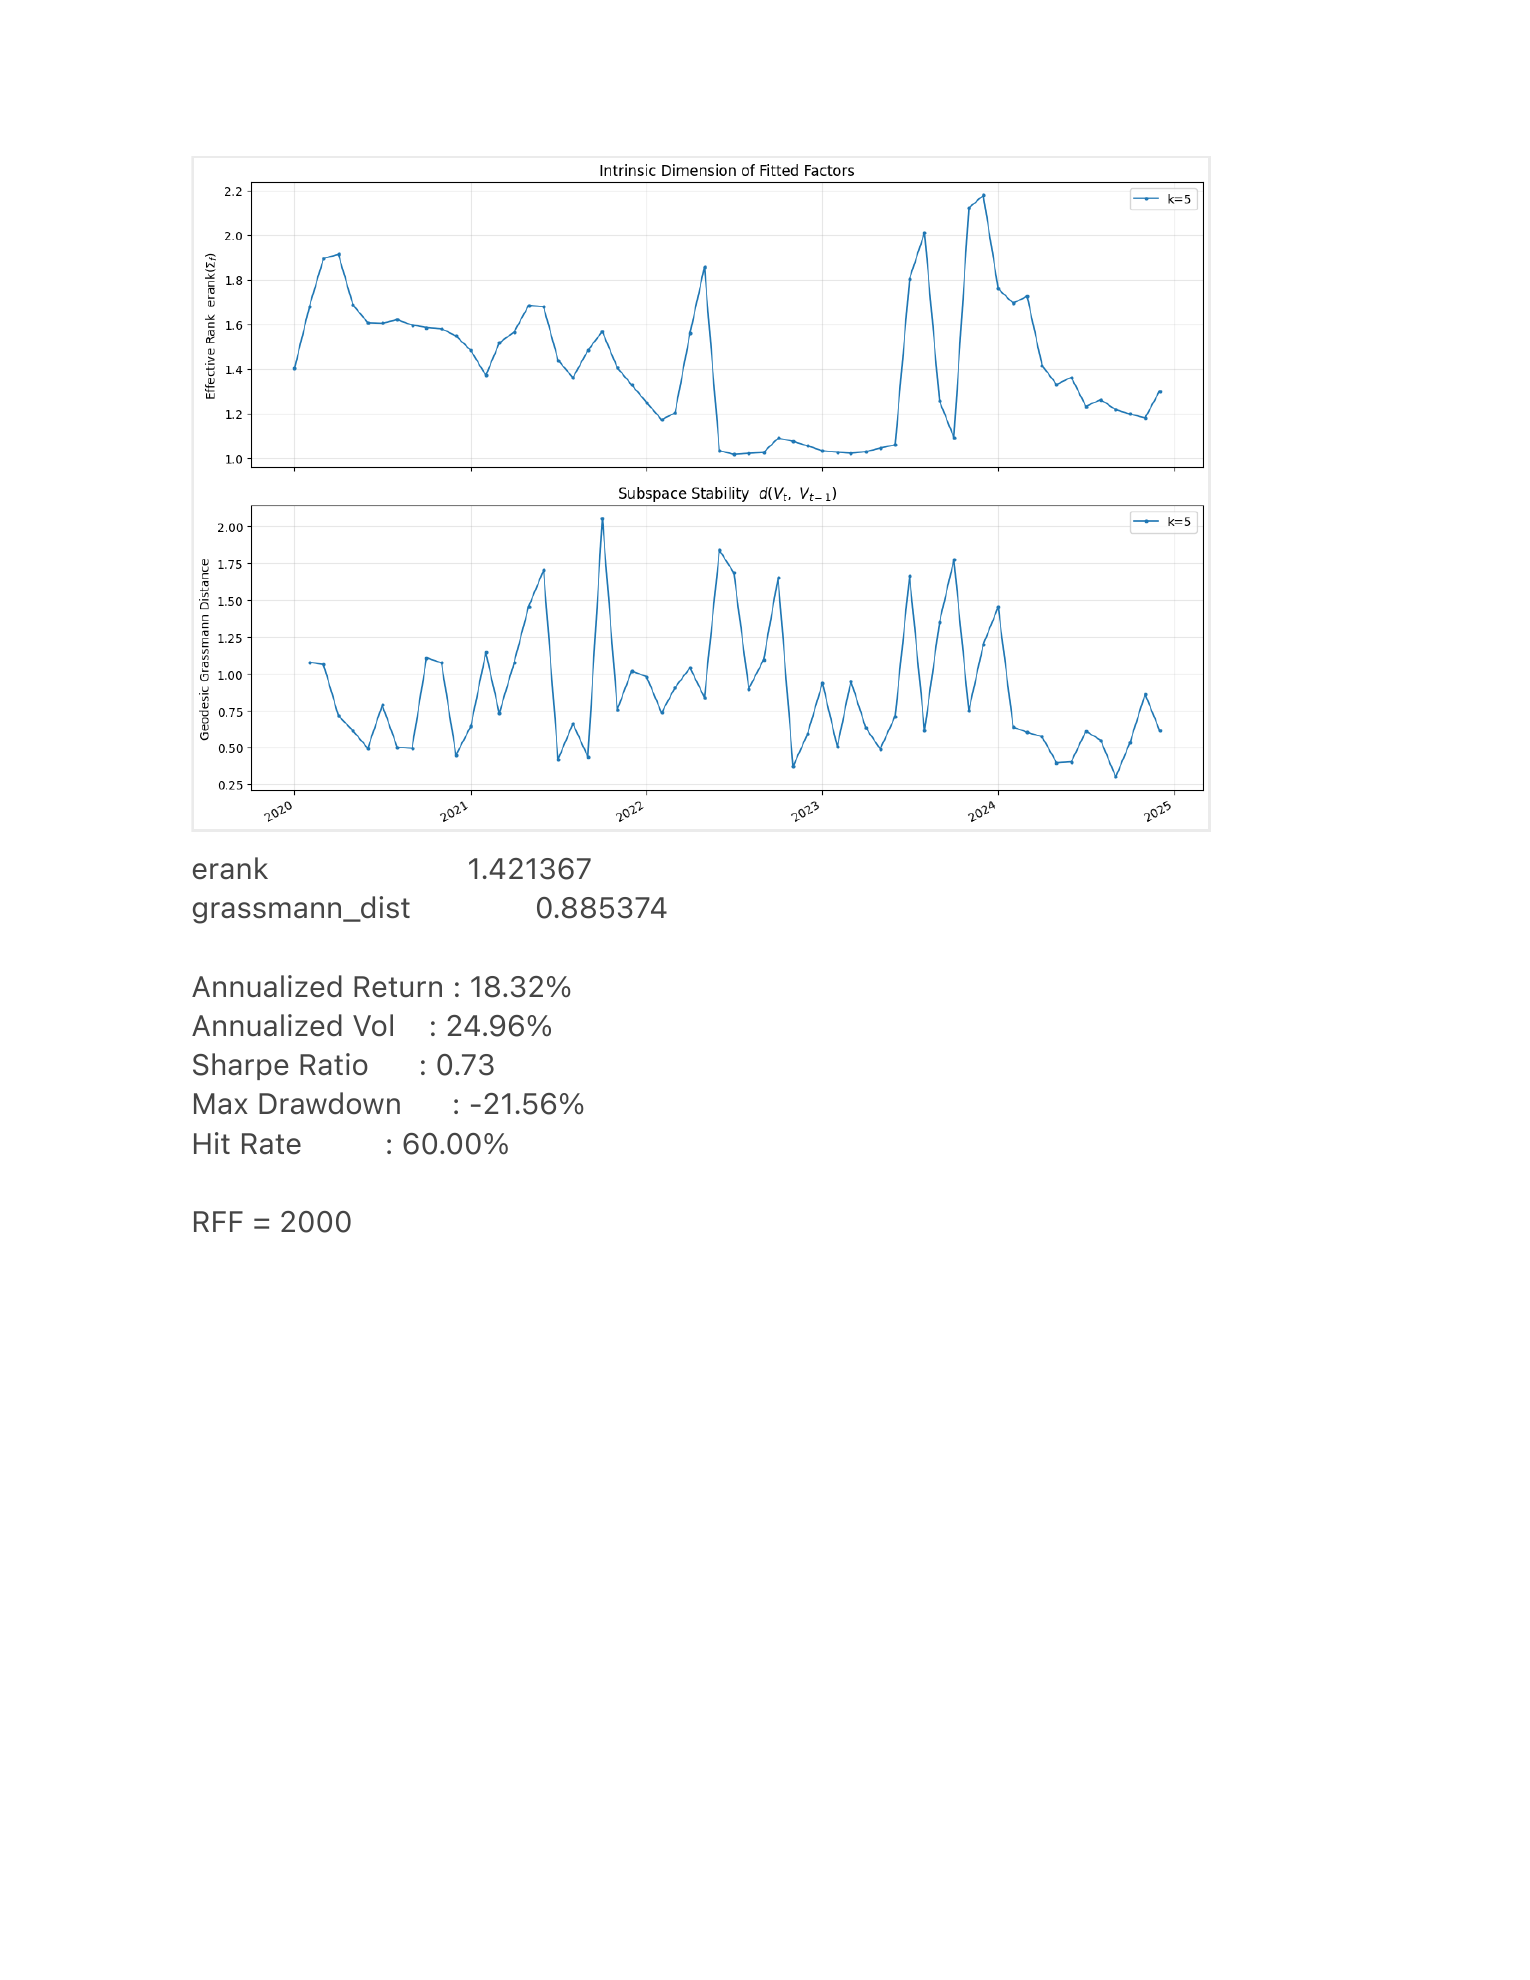
\includegraphics[width=0.88\textwidth]{figures/results_page2.png}
\caption{Extracted panel from the uploaded PDF: baseline / no-RFF summary.}
\end{figure}

\begin{figure}[H]
\centering
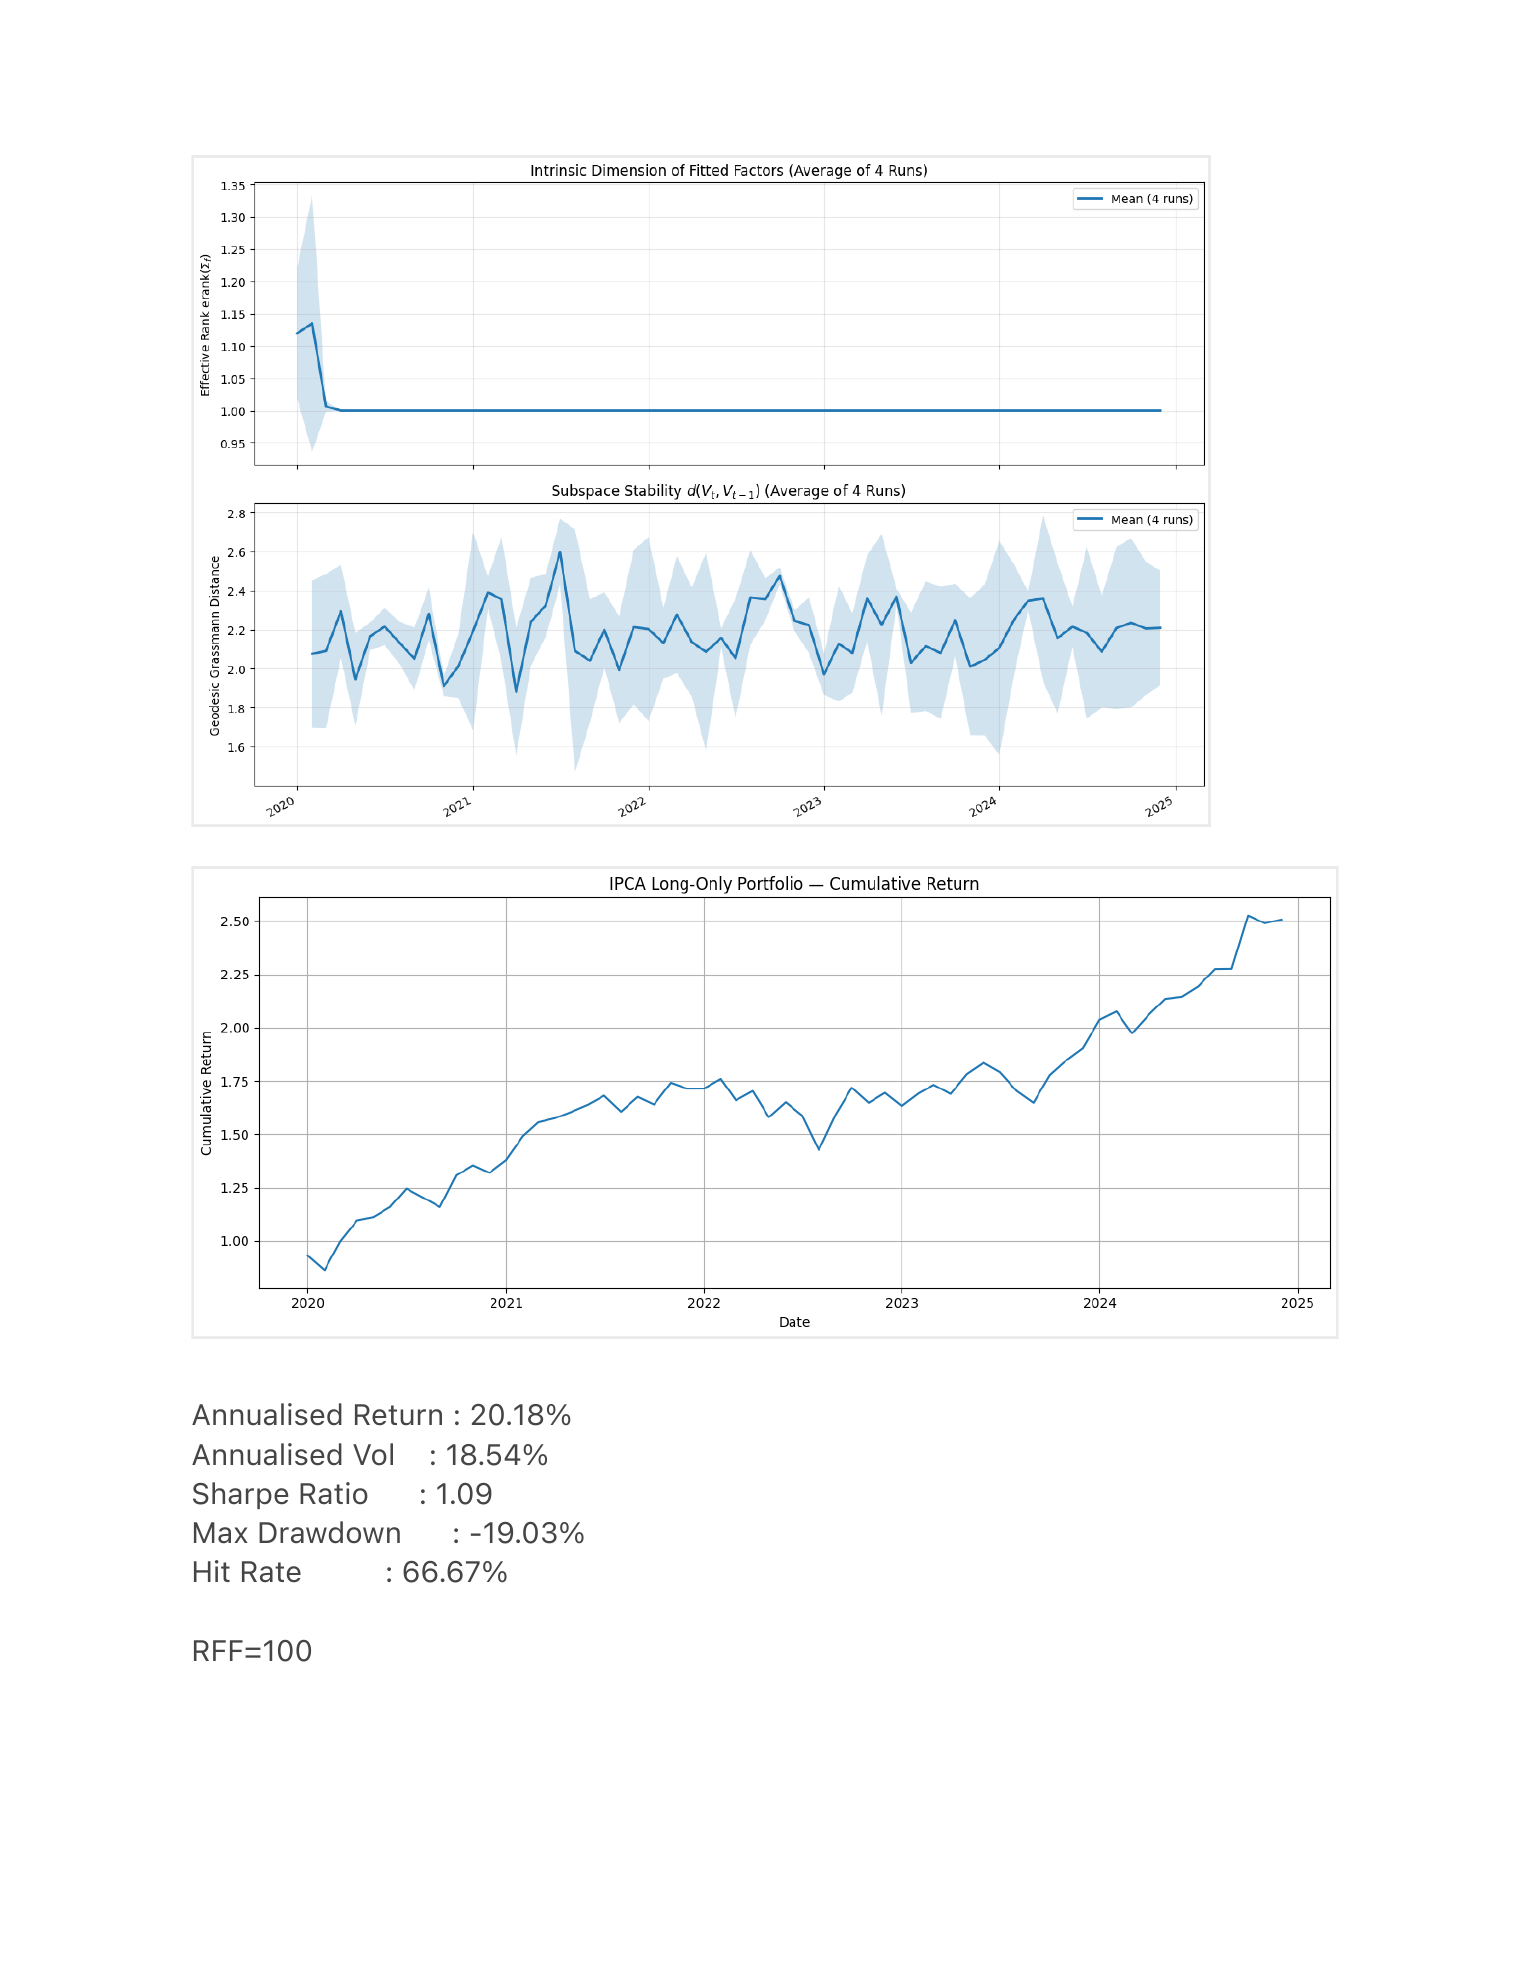
\includegraphics[width=0.88\textwidth]{figures/results_page3.png}
\caption{Extracted panel from the uploaded PDF: RFF = 2000 summary.}
\end{figure}

\begin{figure}[H]
\centering
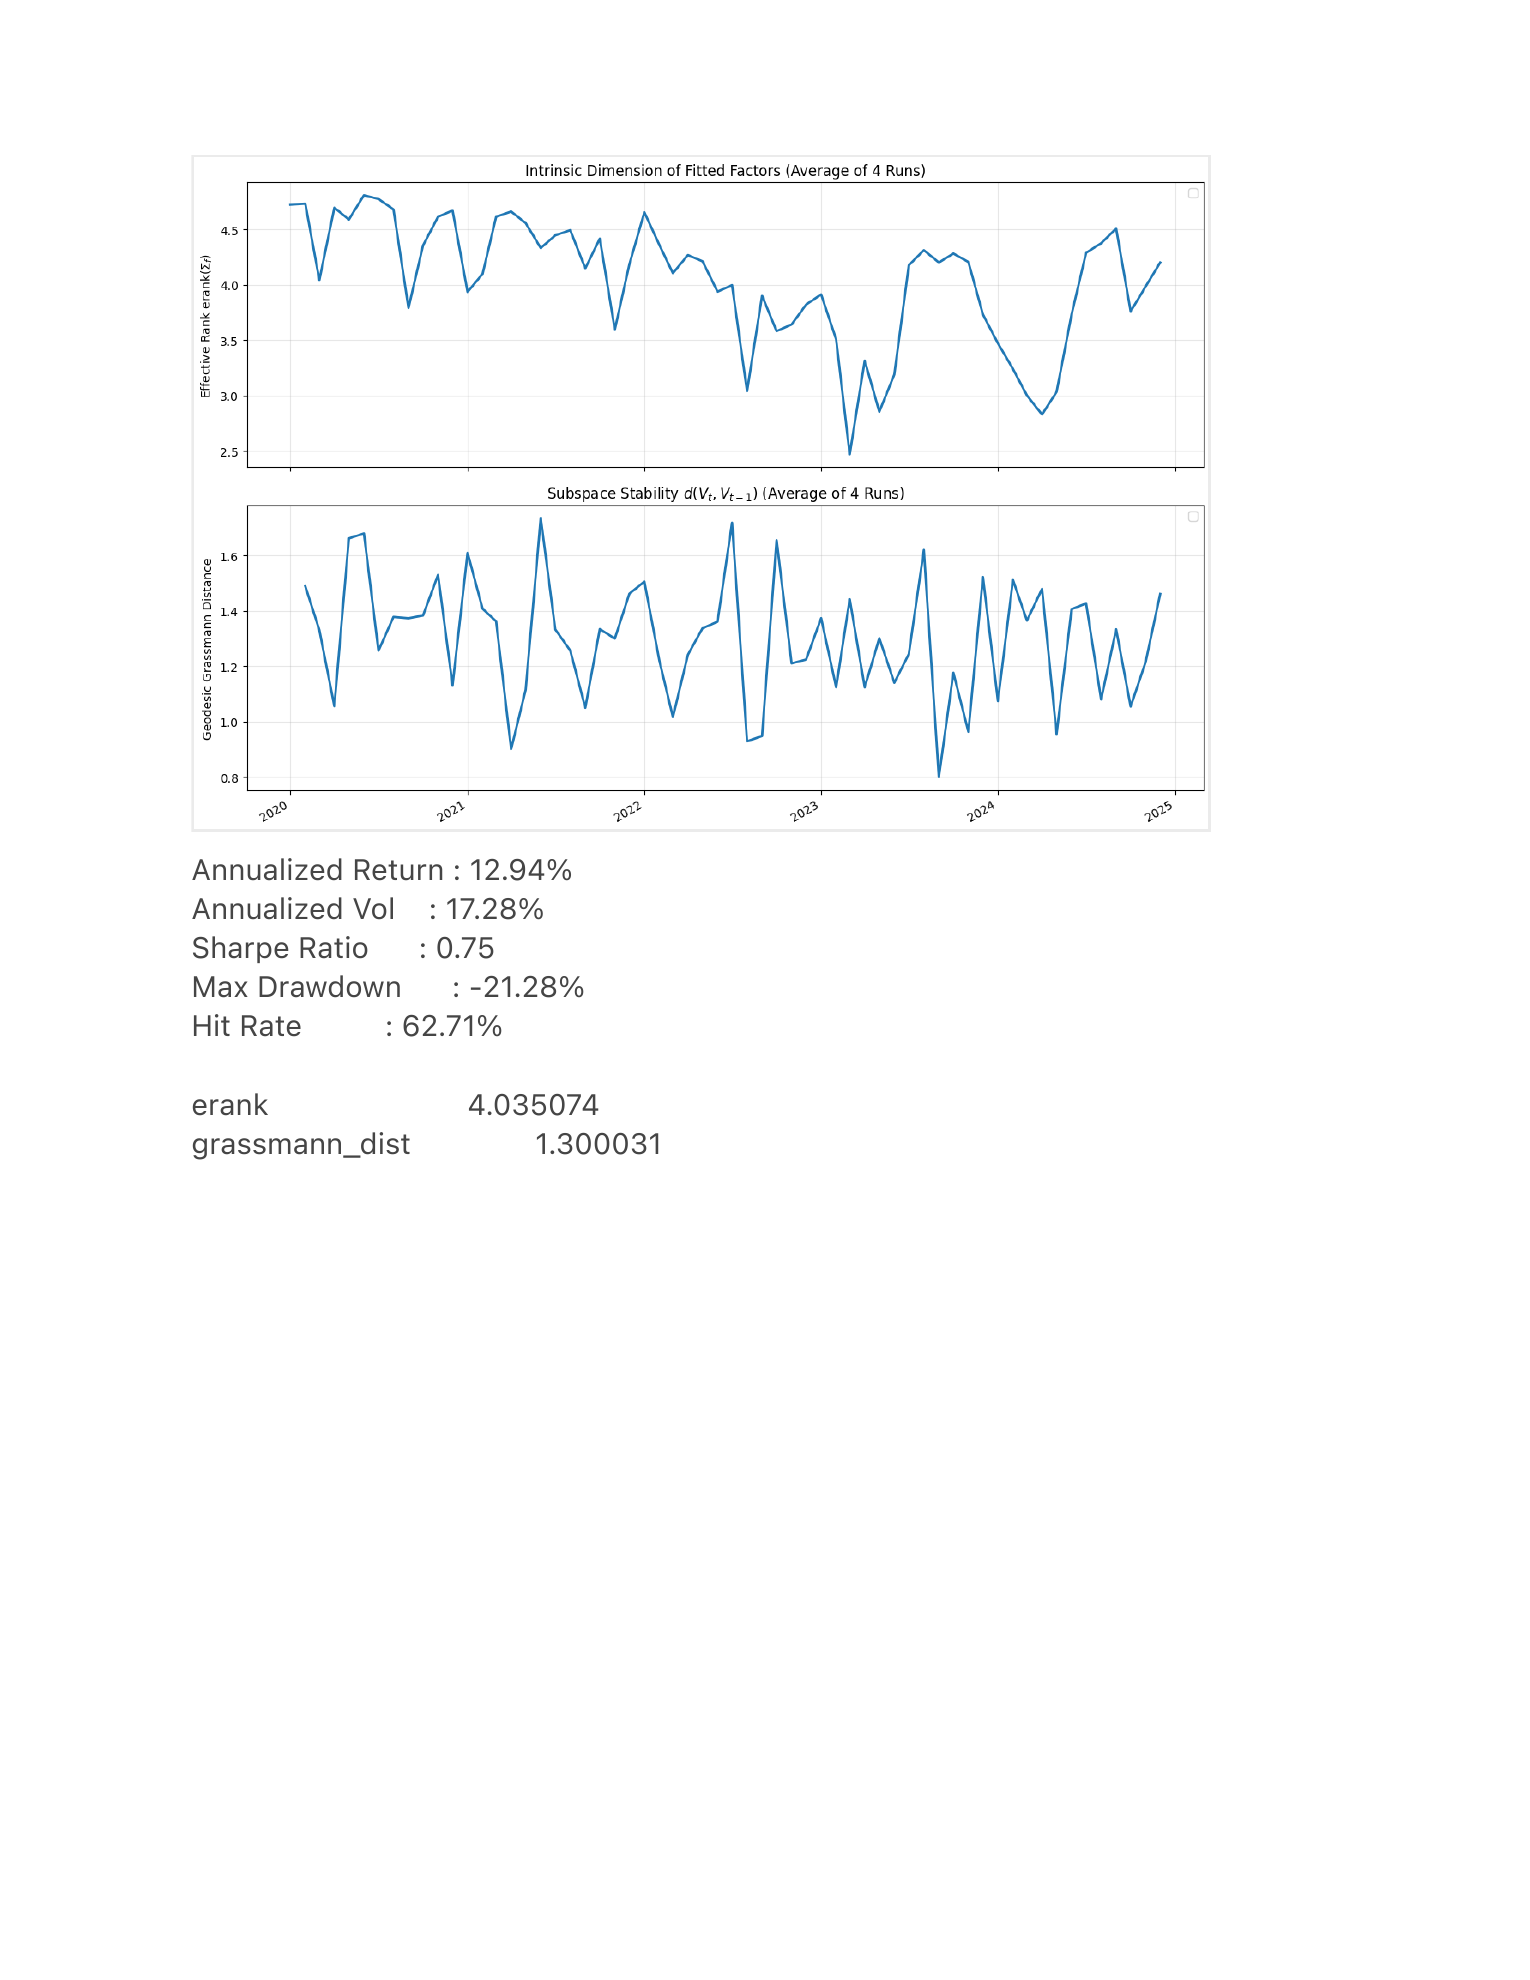
\includegraphics[width=0.88\textwidth]{figures/results_page4.png}
\caption{Extracted panel from the uploaded PDF: RFF = 100 summary.}
\end{figure}

\section{Rolling-window Grassmann diagnostics}

The strongest geometric evidence comes from the rolling-window plots.
These are important because they reveal whether the estimated subspaces are merely fitting well in aggregate,
or whether they remain stable through time.

\subsection{RFF = 1000}
The RFF = 1000 rolling plot is especially useful because it combines the two objects that matter most:
effective rank and Grassmann distance. In the uploaded figure, effective rank stays in a fairly narrow band,
but Grassmann distance remains elevated. That is evidence of persistent subspace rotation even when performance is decent.

\begin{figure}[H]
\centering
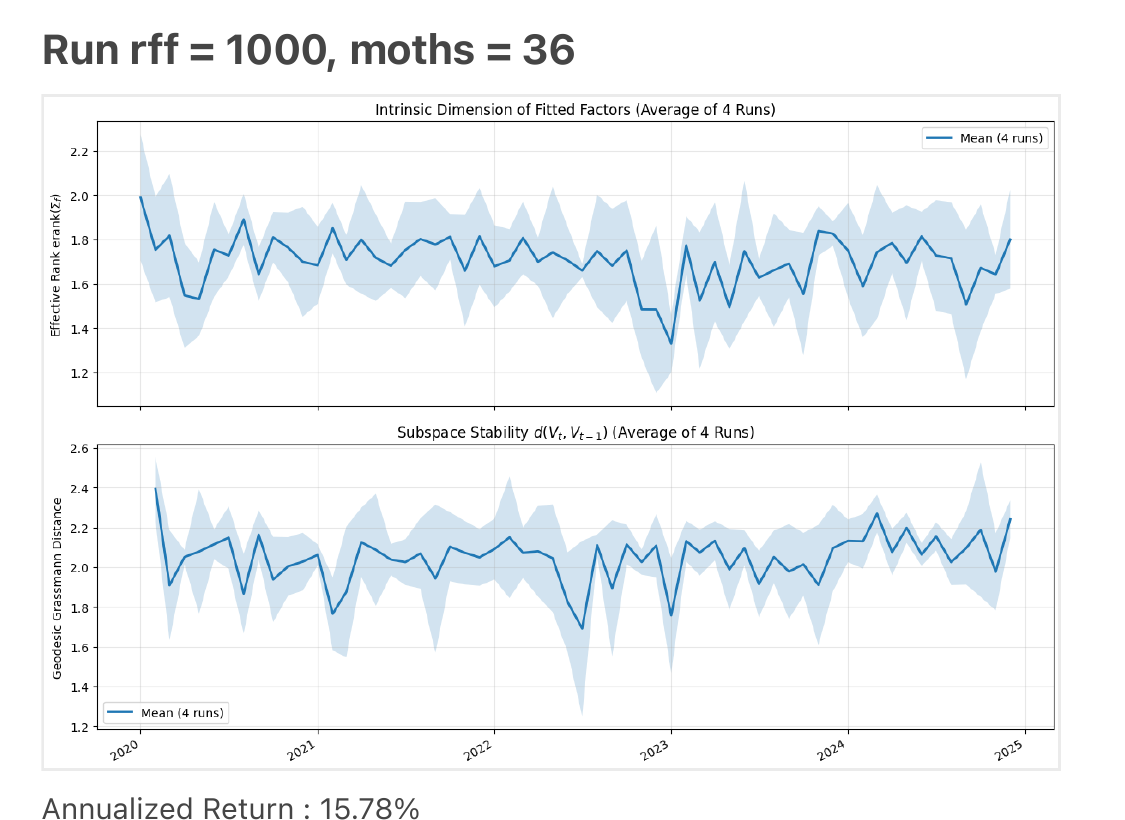
\includegraphics[width=0.96\textwidth]{figures/rff1000_roll.png}
\caption{Rolling effective-rank and Grassmann-distance diagnostics for RFF = 1000. This is the cleanest direct evidence that improved performance does not necessarily imply subspace stability.}
\end{figure}

\begin{figure}[H]
\centering
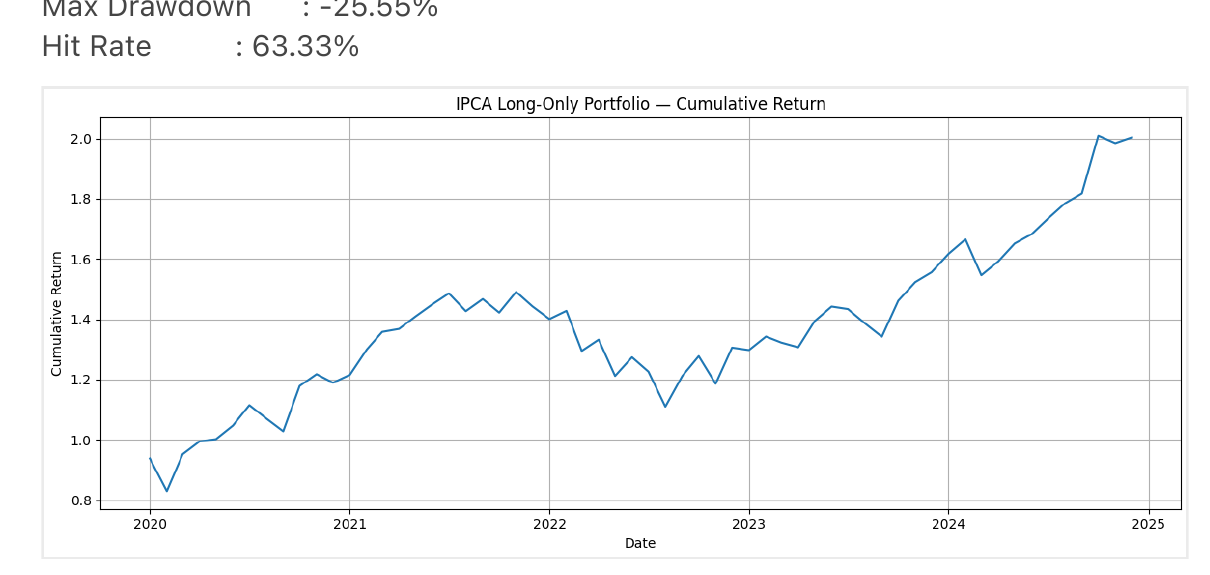
\includegraphics[width=0.78\textwidth]{figures/rff1000_cum.png}
\caption{Cumulative return path for the RFF = 1000 specification. Performance compounds well despite the elevated rolling Grassmann distance.}
\end{figure}

\subsection{Baseline and lower-complexity comparison}
The next two figures help explain the tradeoff. Without RFF, the system is simpler and Grassmann movement is more limited.
At RFF = 100, effective rank is relatively high, which suggests that the added flexibility is actually spreading across more active directions.
By RFF = 1000, however, the span appears less intrinsically rich and more rotationally unstable.

\begin{figure}[H]
\centering
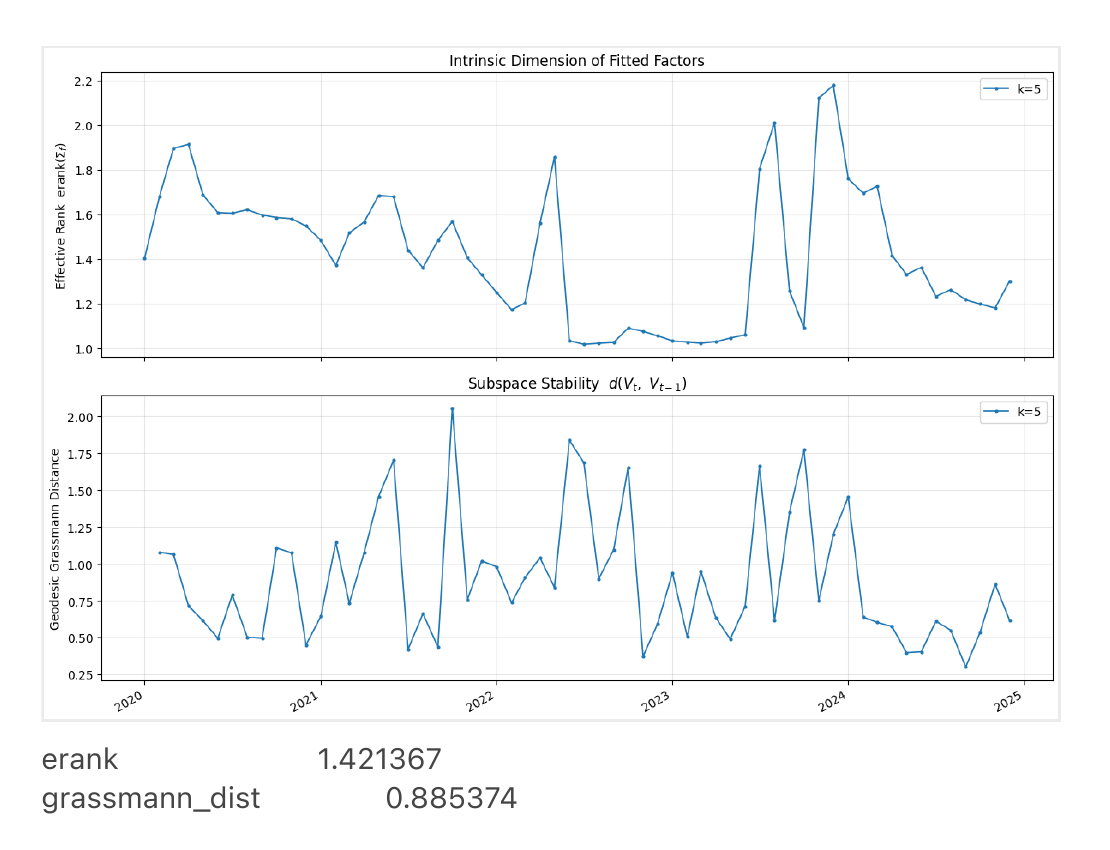
\includegraphics[width=0.95\textwidth]{figures/norrff_roll.png}
\caption{Rolling diagnostics for the no-RFF baseline.}
\end{figure}

\begin{figure}[H]
\centering
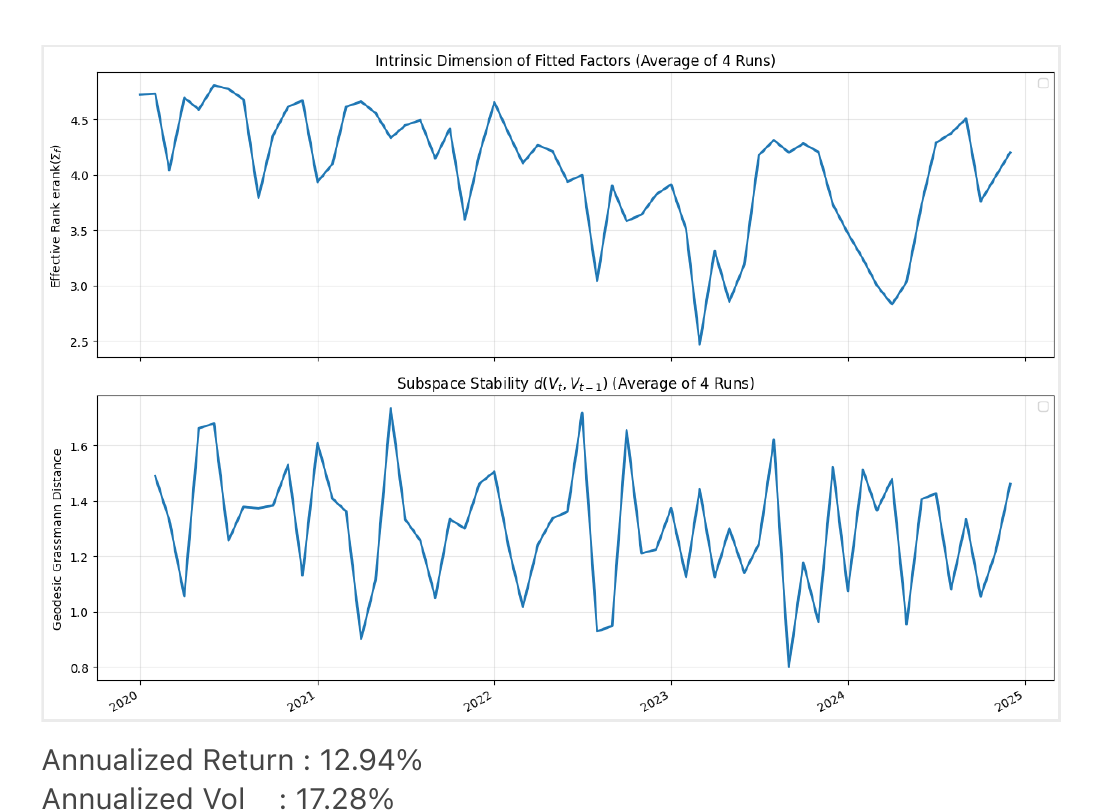
\includegraphics[width=0.95\textwidth]{figures/rff100_roll.png}
\caption{Rolling diagnostics for RFF = 100. This is the configuration with the strongest effective-rank number among the page-level summaries.}
\end{figure}

\begin{figure}[H]
\centering
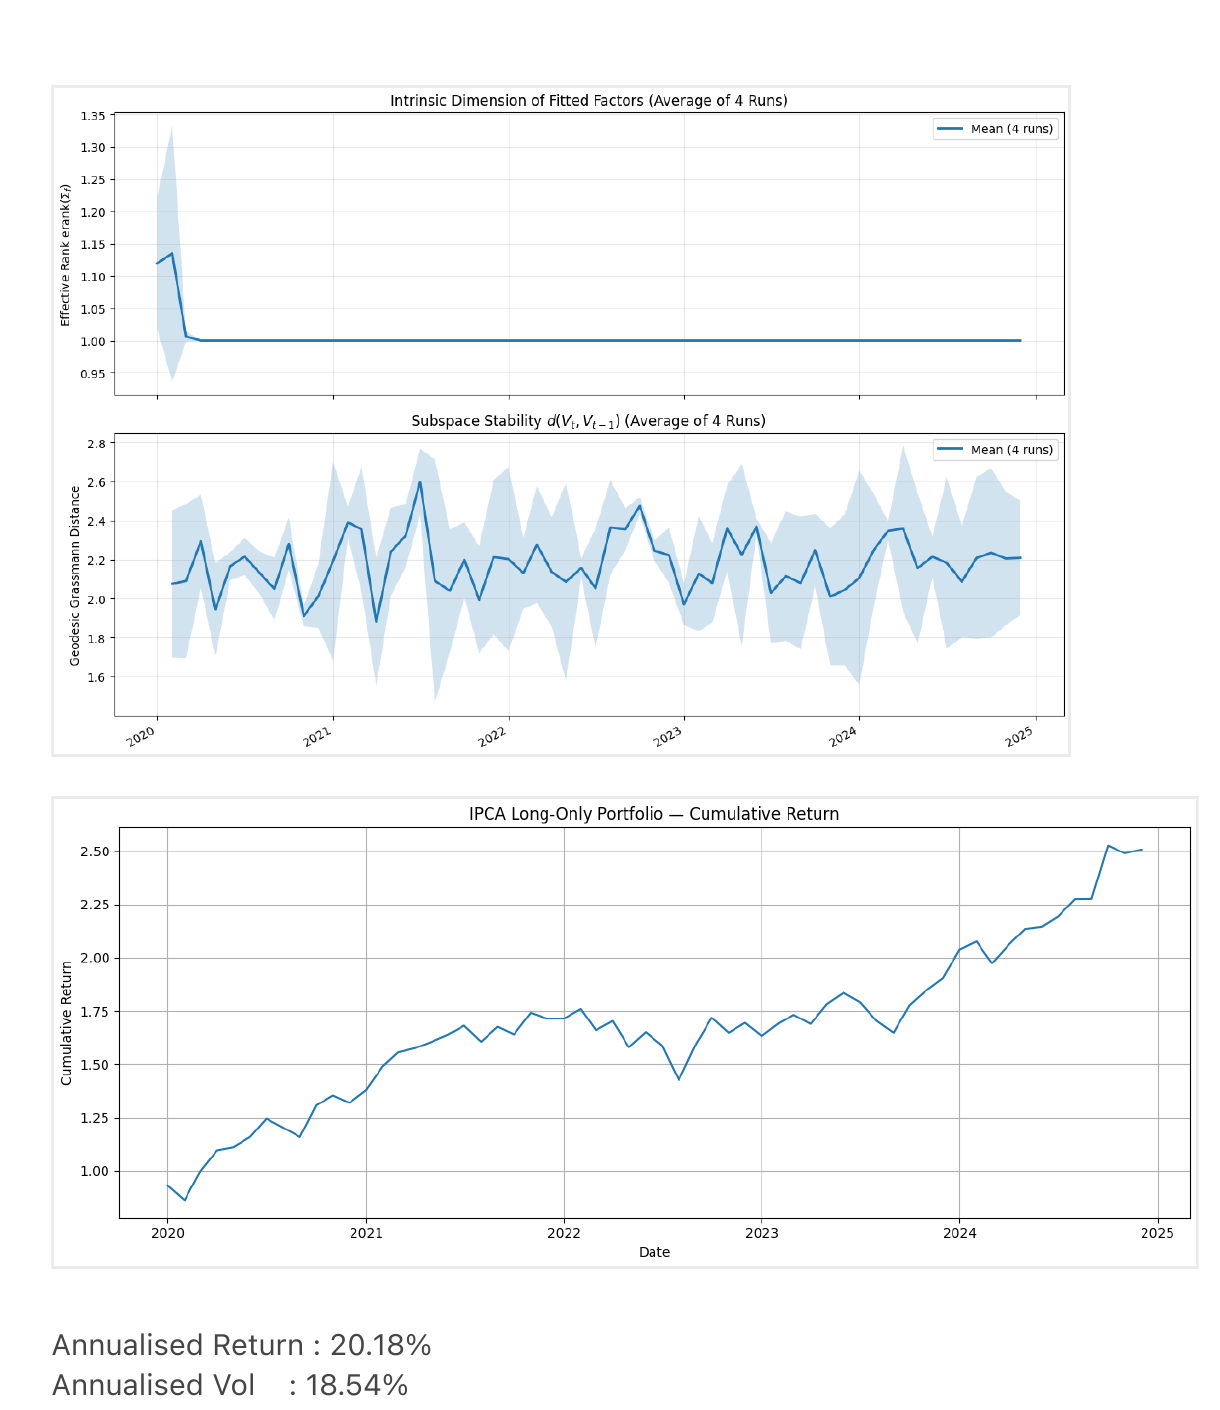
\includegraphics[width=0.95\textwidth]{figures/rff2000_roll_cum.png}
\caption{High-complexity panel for RFF = 2000. This configuration has the strongest Sharpe ratio in the summary results.}
\end{figure}

\section{Supplementary comparison pages}

The remaining two figures are useful as compact references because they place multiple configurations side by side.

\begin{figure}[H]
\centering
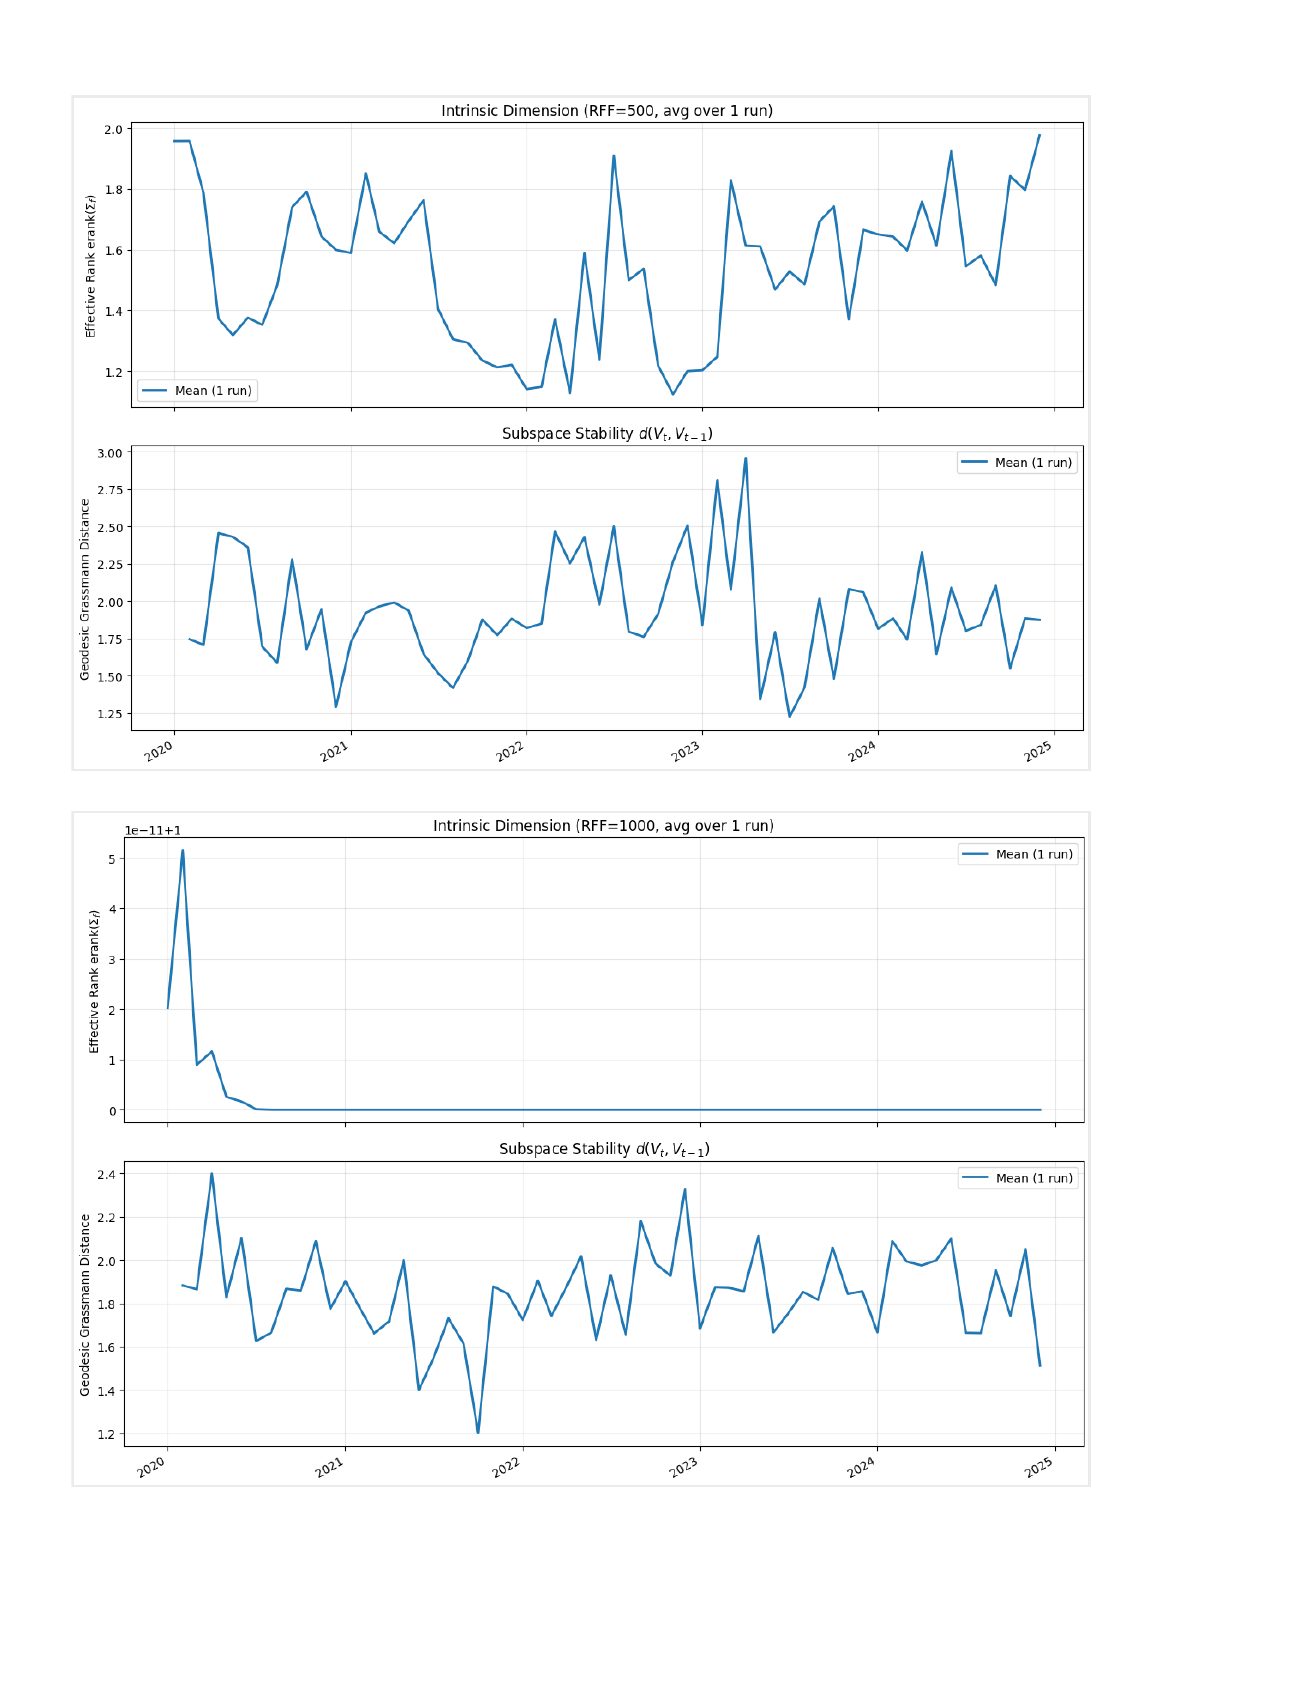
\includegraphics[width=0.96\textwidth]{figures/compare_500_1000.png}
\caption{Side-by-side comparison page for RFF = 500 and RFF = 1000.}
\end{figure}

\begin{figure}[H]
\centering
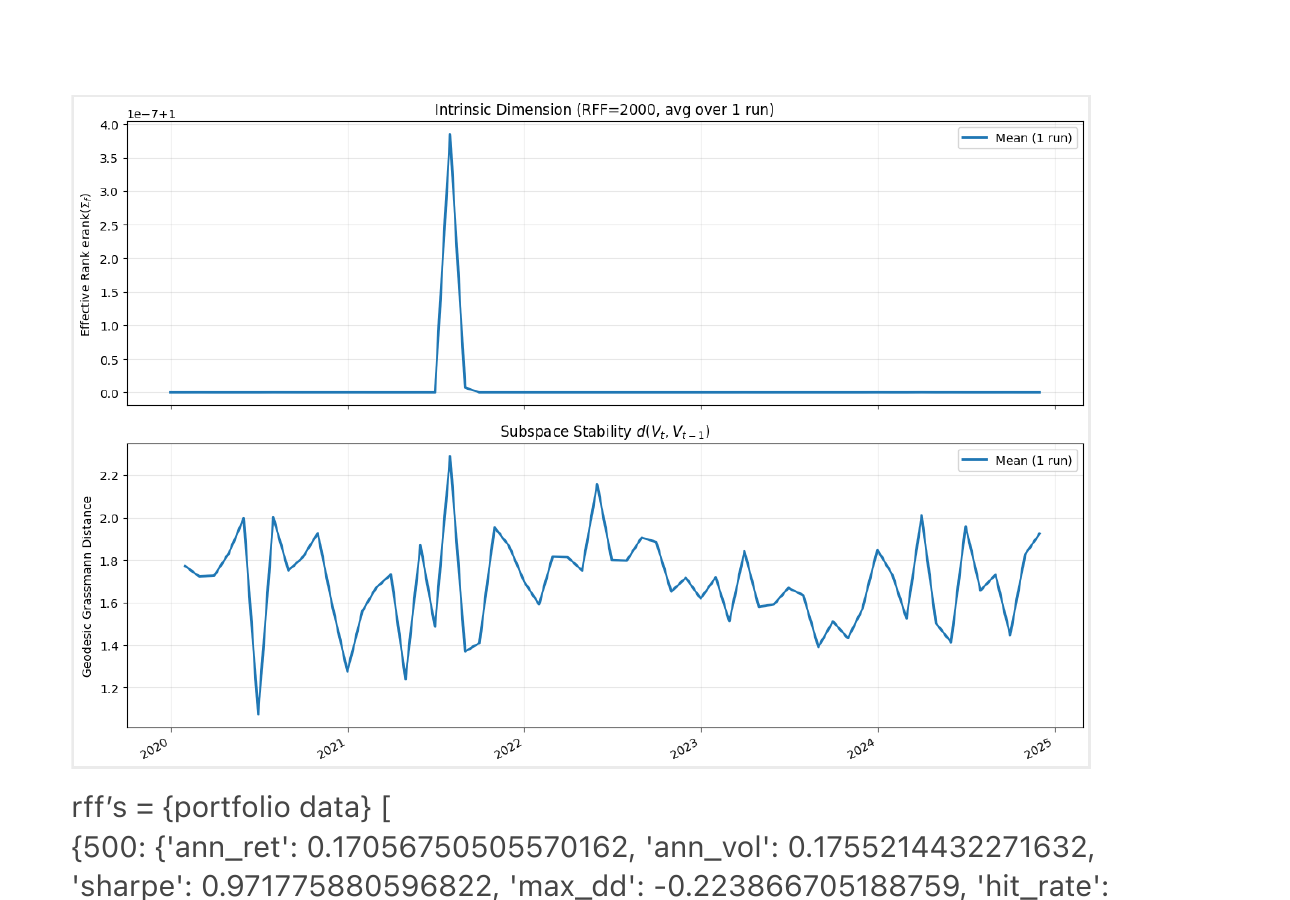
\includegraphics[width=0.96\textwidth]{figures/compare_2000_summary.png}
\caption{One-run summary page for RFF = 2000.}
\end{figure}

\section{Connection to the Virtue of Complexity}

The uploaded results are aligned with the broad message of the virtue-of-complexity literature.
Higher nonlinear complexity can improve out-of-sample Sharpe ratio because it expands approximation power and allows the model
to capture richer conditional structure than a linear or low-dimensional alternative.

So on the \emph{performance} dimension, the evidence is straightforward:
\begin{itemize}
    \item No RFF: Sharpe $\approx 0.73$
    \item RFF = 100: Sharpe $\approx 0.75$
    \item RFF = 1000: Sharpe $\approx 0.82$
    \item RFF = 2000: Sharpe $\approx 1.09$
\end{itemize}

That progression is difficult to dismiss. It says the nonlinear lifting is economically valuable.

\section{Connection to Grassmann geometry}

The geometry paper introduces a different standard for evaluating complexity.
The issue is not only whether richer models fit or trade better, but whether they identify a \emph{stable} and \emph{persistent}
trajectory of return subspaces.

Under that lens, the evidence here is more mixed:
\begin{itemize}
    \item effective rank is not monotone in complexity,
    \item rolling Grassmann distance can increase materially,
    \item the strongest performance setting may still be geometrically unstable.
\end{itemize}

This means some of the additional nonlinear flexibility may be \emph{structurally meaningful}, while some may be \emph{illusory}:
it improves fit or trading performance, but through directions that are weakly identified and rotate under perturbation.

\section{Why standard Kelley IPCA is not a good option here}

This is the core research conclusion.

Standard IPCA estimates a parameter matrix and latent factors through a least-squares criterion. In a high-dimensional lifted feature space,
that creates a serious identification problem:
\begin{itemize}
    \item many different parameter matrices can induce nearly the same fitted return span,
    \item the objective becomes flat in directions that rotate the span inside weakly identified eigenspaces,
    \item optimization can therefore look numerically successful while the underlying parameterization remains unstable.
\end{itemize}

In other words, \textbf{the estimator is solving for the wrong object}. The economically meaningful object is the induced return span,
not the raw loading matrix.

That is exactly why the uploaded rolling Grassmann plots are so useful. They show that even when cumulative returns look good,
the subspaces can still move around materially. So the issue is not that Kelley IPCA cannot produce a fit.
It clearly can. The issue is that in this regime the fitted coefficients are not the right thing to interpret or stabilize.

A sharper way to say it is:

\begin{quote}
\emph{In a high-dimensional RFF lift, standard Kelley IPCA can be economically successful but geometrically unstable.
That makes it a poor estimator for ``stable IPCA'' even when its out-of-sample Sharpe ratio looks strong.}
\end{quote}

\section{What a better framing looks like}

A Grassmann-based framing asks for three diagnostics jointly:
\begin{enumerate}
    \item out-of-sample performance,
    \item intrinsic dimension (effective rank),
    \item rolling subspace stability (Grassmann distance).
\end{enumerate}

That combined view is much stronger than using Sharpe alone. It lets you say:
\begin{itemize}
    \item complexity is \textbf{economically virtuous} when Sharpe improves,
    \item complexity is \textbf{geometrically virtuous} only when that improvement comes with persistent, stable span expansion.
\end{itemize}

Your uploaded results support the first statement strongly, but support the second only partially.
That is exactly why a Grassmann estimator or a Grassmann comparison framework is more defensible than a raw Kelley-IPCA coefficient analysis.

\section{Bottom line}

The package can be summarized in one sentence:

\begin{quote}
\textbf{The uploaded RFF--IPCA results support the virtue of complexity in portfolio performance, but the rolling Grassmann plots show that the added nonlinear flexibility does not uniformly stabilize the identified return span; therefore standard Kelley IPCA is not a good choice when the goal is stable IPCA in a lifted-feature regime.}
\end{quote}

That is the main takeaway this package is designed to document.

\end{document}
